\chapter{Results}
\label{ch:results}

In this chapter, the results of the analysis are presented. First, I present the results of the
efficiency analysis in \autoref{sec:efficiency_angres}. The initial tests of parameter combinations
are based on a small dataset consisting of \(\num{20}\) runs, \ie \(\num{12668}\) events. This is
due to the number of parameter combinations that are tested, as more runs would increase the
processing time immensely. Furthermore, I show the results of the angular resolution for a combined
metric with the efficiency. Then, in \autoref{sec:metrics}, the metrics of each resulting combination
of hyperparameters are plotted. In \autoref{sec:performance}, the performance of each cleaning
algorithm compared to the default settings is shown. Finally, a comparison of the different
cleaning algorithms is provided in \autoref{sec:comparison}.


\section{Analysis of the Efficiency and the Angular Resolution}
\label{sec:efficiency_angres}

To narrow down possible candidates for the optimal hyperparameters, I first analyzed the efficiency
of the different cleaning algorithms. The efficiency is determined by the number of events that are
reconstructed after cleaning. For this work I chose \(\num{20}\) intervals within \(\num{0}\) and
\(\num{1}\) with a step size of \(\num{0.05}\). The number of reconstructed events \(n_{\mathrm{reco}}\)
and the total number of events \(n_{\mathrm{total}}\) are binned per energy and the efficiency is then
calculated as
\begin{equation}\label{eq:efficiency_sum}
    \eff = \frac{\sum_{N} n_{\mathrm{reco}}}{\sum_{\mathrm{N}} n_{\mathrm{total}}},
\end{equation}
with \(N\) being the number of bins. For each interval only those datasets are selected, where the efficiency
lies between the lower and upper bound of the interval. Then the minimum angular resolution is
determined for each interval. The parameters of these datasets are then selected to be the optimal
parameters for each cleaning algorithm. This not only allows for a comparison of the cleaners but also
a decision on a trade-off between the efficiency and the angular resolution, namely having a better
angular resolution, but a lower efficiency, or a higher efficiency but also a higher and therefore worse
angular resolution. The results for the efficiency are listed in \autoref{tab:efficiency} and
the results for the mean angular resolution in \autoref{tab:angres}.

As one can see, not all cleaning algorithms have valid values for each interval, peaking at a maximum
of around \(\SIrange{40}{45}{\percent}\) of successfully reconstructed events. This is because not
all events are stereo events, \ie events, where two or more telescopes were triggered, which is a
requirement for the reconstruction.
The remaining events are therefore mono events and do not contribute to either the efficiency or the
angular resolution. The efficiency would be higher, of course, for a full-array analysis, but that would
mean also including \glspl{lst} data\footnote{which was left out due to time limitations, see \autoref{ch:conclusions}.},
which for this work would not help find the optimal parameters, since it is better to analyze the telescope
types separately. The reason for the latter is, that optimizing the telescopes by type would lead to
better results for the hyperparameters for the respective telescopes.
\begin{table}
    \centering
    \caption{The results of the analysis for the efficiency of each cleaning algorithm taken over all
    energy bins. The table lists the lower and upper limits of each efficiency
    interval. The efficiency is calculated according to \autoref{eq:efficiency_sum} and
    each listed efficiency is the one where the mean angular resolution is minimal for the given
    interval. Notice how not all cleaning algorithms have valid results for all efficiency intervals, due to not all
    events being stereo events.}
    \label{tab:efficiency}
    \rowcolors{0}{white!92!black}{}
    \begin{tabular}{S[table-format=1.2] S[table-format=1.2] S[table-format=1.3] S[table-format=1.3] S[table-format=1.3] S[table-format=1.3]}
        \hiderowcolors
        & & \multicolumn{4}{c}{Efficiency} \\
        {$\eff_{\mathrm{lower}}$} & {$\eff_{\mathrm{upper}}$} & {Tailcuts} & {MARS} & {FACT} & {TCC} \\
        \addlinespace[0.5em]
        \showrowcolors
        % \input{build/efficiency.txt}
        0.00 & 0.05 &       &       & 0.007 &       \\
        0.05 & 0.10 &       &       & 0.051 & 0.070 \\
        0.10 & 0.15 & 0.121 & 0.122 & 0.141 & 0.121 \\
        0.15 & 0.20 & 0.177 & 0.179 & 0.178 & 0.176 \\
        0.20 & 0.25 & 0.242 & 0.244 & 0.250 & 0.248 \\
        0.25 & 0.30 & 0.296 & 0.297 & 0.254 & 0.263 \\
        0.30 & 0.35 & 0.307 & 0.306 & 0.340 & 0.311 \\
        0.35 & 0.40 & 0.365 & 0.380 & 0.388 & 0.375 \\
        0.40 & 0.45 & 0.401 & 0.410 & 0.405 & 0.401 \\
    \end{tabular}
\end{table}

\begin{table}
    \centering
    \caption{The results of the analysis for the mean angular resolution of each cleaning algorithm.
    The table lists the lower and upper limits of each efficiency interval. The angular resolution listed
    is the minimum mean angular resolution of the respective efficiency interval. The corresponding efficiency
    values are listed in \autoref{tab:efficiency}. Notice how not all cleaning algorithms have valid results for all efficiency intervals, due to not all
    events being stereo events.}
    \label{tab:angres}
    \rowcolors{0}{white!92!black}{}
    \begin{tabular}{S[table-format=1.2] S[table-format=1.2] S[table-format=1.3] S[table-format=1.3] S[table-format=1.3] S[table-format=1.3]}
        \hiderowcolors
        & & \multicolumn{4}{c}{Mean Angular Resolution\(\;/\; \si{\degree}\)} \\
        {$\eff_{\mathrm{lower}}$} & {$\eff_{\mathrm{upper}}$} & {Tailcuts} & {MARS} & {FACT} & {TCC} \\
        \addlinespace[0.5em]
        \showrowcolors
        % \input{build/angular_resolution.tex}
        0.00 & 0.05 &       &       & 0.244 &       \\
        0.05 & 0.10 &       &       & 0.428 & 0.413 \\
        0.10 & 0.15 & 0.358 & 0.291 & 0.415 & 0.396 \\
        0.15 & 0.20 & 0.308 & 0.282 & 0.367 & 0.340 \\
        0.20 & 0.25 & 0.334 & 0.332 & 0.403 & 0.388 \\
        0.25 & 0.30 & 0.346 & 0.356 & 0.366 & 0.386 \\
        0.30 & 0.35 & 0.357 & 0.343 & 0.365 & 0.383 \\
        0.35 & 0.40 & 0.395 & 0.395 & 0.404 & 0.390 \\
        0.40 & 0.45 & 0.432 & 0.424 & 0.420 & 0.427 \\
    \end{tabular}
\end{table}
The results listed in the tables show that there is a clear trade-off in choosing between efficiency and angular resolution.
As such, for further comparison of the cleaning algorithms, the corresponding datasets for the efficiency and
the angular resolution are plotted in \autoref{fig:efficiency_angres} for the intervals
\([\num{0.10}, \num{0.15}]\) and \([\num{0.40}, \num{0.45}]\). The reason for this is, that these are
the minimum and maximum intervals \wrt the efficiency, where all cleaners have valid values.
Furthermore, the mean angular resolution is plotted against the efficiency in \autoref{fig:ar_vs_eff}.
\vspace{-0.2cm}
\begin{figure}
    \centering
    \begin{subfigure}{0.48\textwidth}
        \centering
        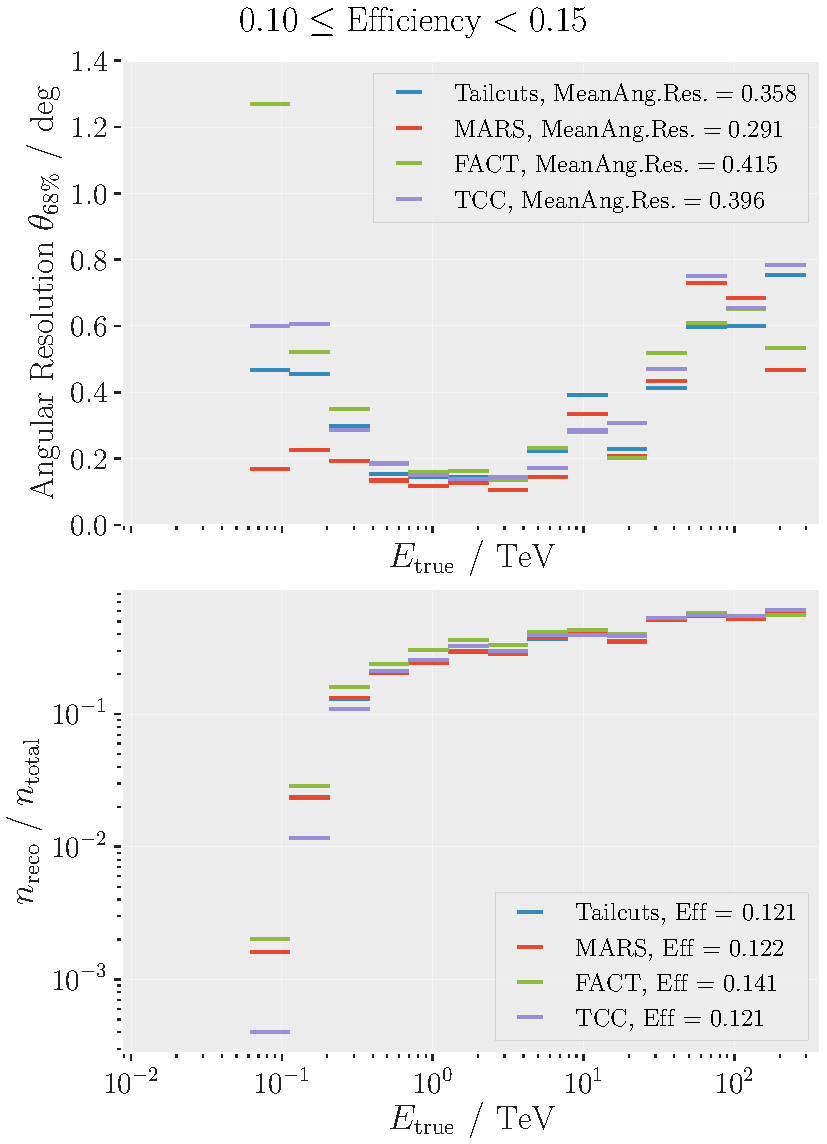
\includegraphics[width=0.8\textwidth]{plots/ar_aeff/AR_Aeff_MST_0.10_0.15.pdf}
    \end{subfigure}
    \hfill
    \begin{subfigure}{0.48\textwidth}
        \centering
        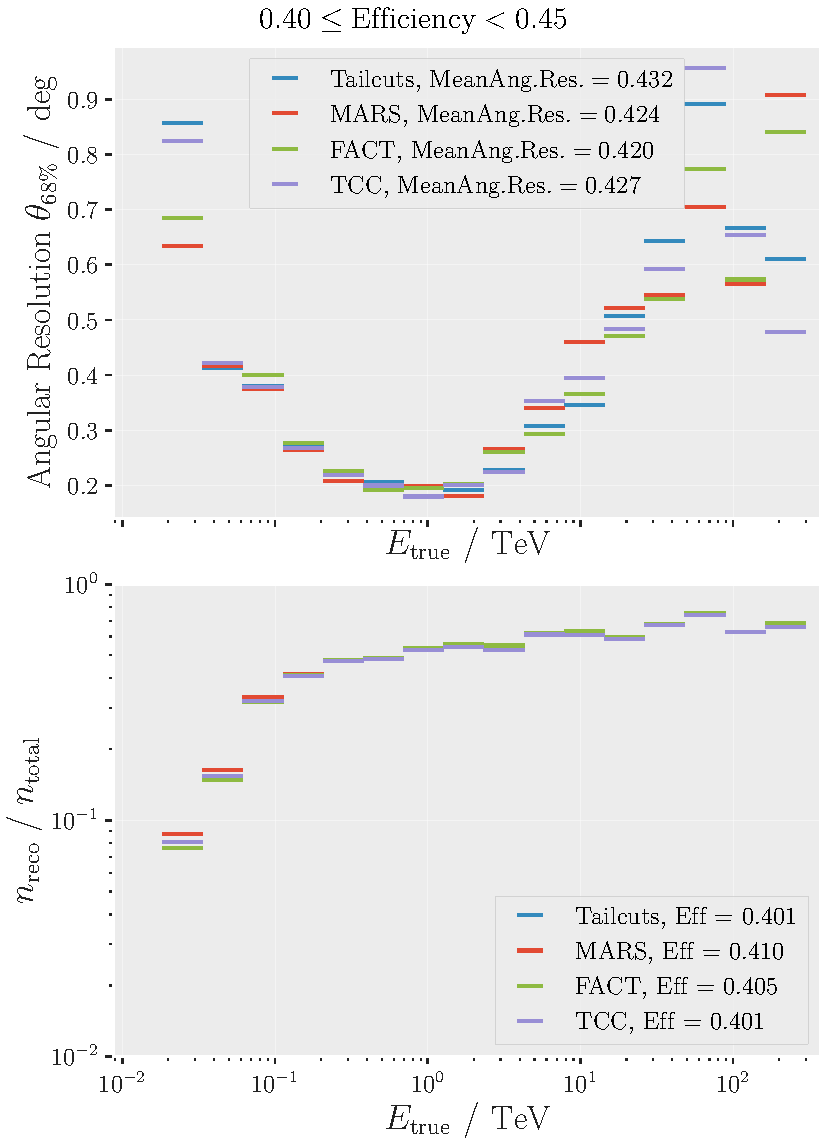
\includegraphics[width=0.8\textwidth]{plots/ar_aeff/AR_Aeff_MST_0.40_0.45.pdf}
    \end{subfigure}
    \caption{Mean angular resolution and efficiency for the MST simulation binned per energy. Notice
    the decrease in the scattering of the mean angular resolution and the efficiency at medium to
    medium-high energies at higher efficiencies in the plots on the right.\vspace{-0.5cm}}
    \label{fig:efficiency_angres}
\end{figure}
\begin{figure}[!htbp]
    \centering
    \includegraphics[width=0.6\textwidth]{build/ar_vs_eff.pdf}
    \caption{Mean angular resolution plotted against the efficiency between \(\num{0.00}\) and \(\num{0.45}\) for
    all for cleaning algorithms. For further analysis, I choose the efficiency over the angular resolution
    as this would leave me with more reconstructed events and thus more statistics. This, however, results in
    a higher and therefore worse angular resolution compared to \eg the values around an efficiency of \(0.18\).}
    \label{fig:ar_vs_eff}
\end{figure}


\section{Metrics of the Cleaning Algorithms}
\label{sec:metrics}
\glsreset{tp}\glsreset{fp}\glsreset{fn}\glsreset{tn}
Concerning the metrics, I first analyzed the parameter combinations of all settings found in \autoref{sec:efficiency_angres}. First,
the number of the \gls{tp}, \gls{fp}, \gls{fn} and \gls{tn} values is calculated per event. Then,
those values are summed up for each setting from the datasets in the previous section and the metrics are calculated as shown in
\autoref{tab:metrics}.

The metrics for each parameter combination are first compared for each cleaning algorithm respectively,
to determine the best setting within a set of parameter combinations. The results are then plotted in
\Autoref{fig:metrics_tail, fig:metrics_mars, fig:metrics_fact, fig:metrics_tcc}
and are shown with specific IDs they were given when the datasets were first processed with \ctapipe.
This improves readability as opposed to writing out the full settings. The hyperparameters for the best performing
IDs of every algorithm are listed in \autoref{tab:best_parameters}.

While all settings perform well w.\,r.\,t., for example, the \gls{tnr}, one can see from the results, that for all cleaning
algorithms, the best parameter combination is the one where the \gls{tpr}, the \gls{acc} and the \gls{ba}
are the highest. These settings are also the ones that correspond to the highest efficiency.
The values for each respective metric and cleaning algorithm are listed in
\Autoref{tab:metrics_tail, tab:metrics_mars, tab:metrics_fact, tab:metrics_tcc} respectively, while
a comparison of the cleaners against each other is shown in \autoref{sec:comparison}.
\begin{table}
    \centering
    \caption{Results for the metrics of \tailcuts{}. One can see, that the best results are obtained
    for the setting with ID~101.}
    \label{tab:metrics_tail}
    \rowcolors{0}{white!92!black}{}
    \adjustbox{varwidth=\linewidth,scale=0.9}{%
    \begin{tabular}{r S[table-format=1.4] S[table-format=1.4] S[table-format=1.4] S[table-format=1.4] S[table-format=1.4] S[table-format=1.4] S[table-format=1.4]}
        \hiderowcolors
        {ID} & \acrshort{tpr} & \acrshort{tnr} & \acrshort{fnr} & \acrshort{acc} & \acrshort{ba} \\
        \addlinespace[0.5em]
        \showrowcolors
        % \input{build/metrics_tail.txt} %% kinda broken atm
        118 & 0.0972 & 1.0000 & 0.9028 & 0.9256 & 0.5486 \\
         51 & 0.1231 & 1.0000 & 0.8769 & 0.9256 & 0.5615 \\
        140 & 0.1460 & 1.0000 & 0.8540 & 0.9256 & 0.5730 \\
        141 & 0.1660 & 1.0000 & 0.8340 & 0.9283 & 0.5830 \\
         81 & 0.1854 & 1.0000 & 0.8146 & 0.9288 & 0.5927 \\
         47 & 0.2268 & 1.0000 & 0.7732 & 0.9332 & 0.6134 \\
        101 & 0.3169 & 0.9997 & 0.6831 & 0.9418 & 0.6583 \\
    \end{tabular}}
\end{table}

\begin{figure}
    \centering
    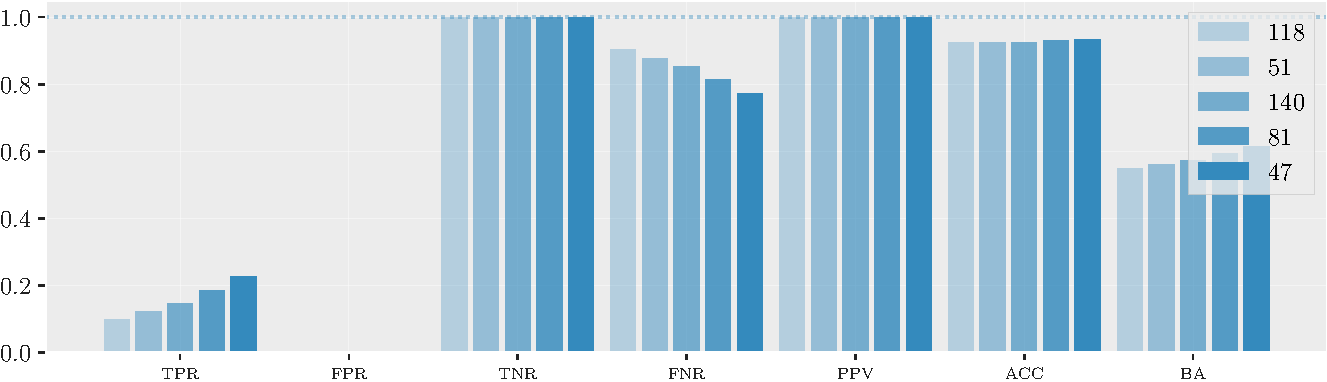
\includegraphics[width=0.95\textwidth]{build/metrics_tailcuts.pdf}
    \caption{Metrics for \tailcuts{}. It can be seen, that the cleaning setting with ID~101 performs
    best in terms of the true positive rate, accuracy and balanced accuracy, making it the best
    setting of the five parameter combinations \wrt the metrics.}
    \label{fig:metrics_tail}
\end{figure}

\begin{table}
    \centering
    \caption{Results for the metrics of \mars{}. The best results \wrt the metrics are obtained
    for the setting with ID~13.}
    \label{tab:metrics_mars}
    \rowcolors{0}{white!92!black}{}
    \begin{tabular}{r S[table-format=1.4] S[table-format=1.4] S[table-format=1.4] S[table-format=1.4] S[table-format=1.4] S[table-format=1.4] S[table-format=1.4]}
        \hiderowcolors
        ID & \acrshort{tpr} & \acrshort{tnr} & \acrshort{fnr} & \acrshort{acc} & \acrshort{ba} \\
        \addlinespace[0.5em]
        \showrowcolors
        % \input{build/metrics_mars.txt}
         54 & 0.1069 & 1.0000 & 0.8931 & 0.9256 & 0.5534 \\
         59 & 0.1369 & 1.0000 & 0.8631 & 0.9256 & 0.5684 \\
         76 & 0.1565 & 1.0000 & 0.8435 & 0.9256 & 0.5782 \\
         60 & 0.1625 & 1.0000 & 0.8375 & 0.9283 & 0.5812 \\
        135 & 0.1738 & 1.0000 & 0.8262 & 0.9607 & 0.5869 \\
         15 & 0.2433 & 1.0000 & 0.7567 & 0.9640 & 0.6216 \\
         13 & 0.3460 & 0.9995 & 0.6540 & 0.9684 & 0.6727 \\
    \end{tabular}
\end{table}

\begin{figure}
    \centering
    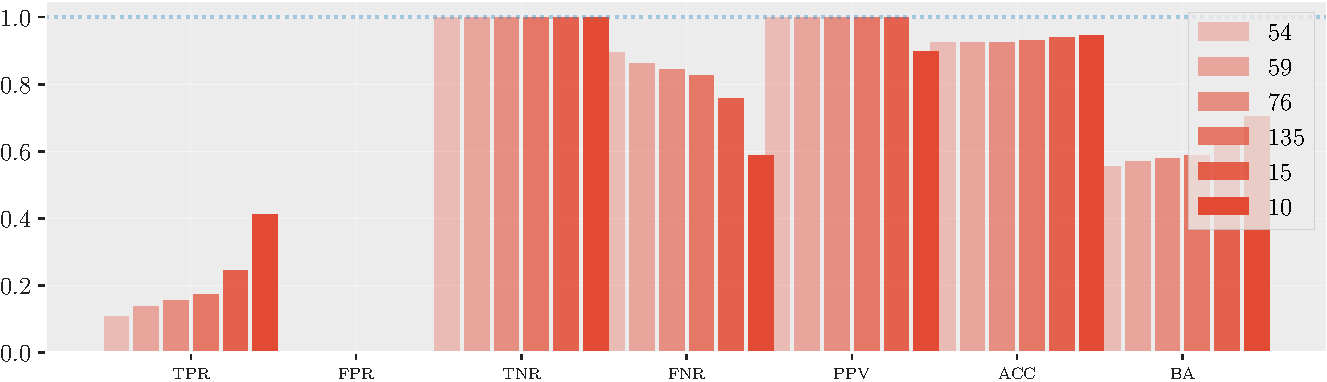
\includegraphics[width=\textwidth]{build/metrics_mars.pdf}
    \caption{Metrics for \mars{}. The results show that the cleaning setting with ID~13 performs
    best in terms of the true positive rate, accuracy and balanced accuracy, making it the best
    setting of the five parameter combinations \wrt the metrics.}
    \label{fig:metrics_mars}
\end{figure}

\begin{table}
    \centering
    \caption{Results for the metrics of \fact{}. One can see, that the best results are obtained
    for the settings with ID~974.}
    \label{tab:metrics_fact}
    \rowcolors{0}{white!92!black}{}
    \begin{tabular}{r S[table-format=1.4] S[table-format=1.4] S[table-format=1.4] S[table-format=1.4] S[table-format=1.4] S[table-format=1.4] S[table-format=1.4]}
        \hiderowcolors
        ID & \acrshort{tpr} & \acrshort{tnr} & \acrshort{fnr} & \acrshort{acc} & \acrshort{ba} \\
        \addlinespace[0.5em]
        \showrowcolors
        % \input{build/metrics_fact.txt}
        553 & 0.0077 & 1.0000 & 0.9923 & 0.9256 & 0.5039 \\
        271 & 0.0396 & 1.0000 & 0.9604 & 0.9256 & 0.5198 \\
        767 & 0.1042 & 1.0000 & 0.8958 & 0.9256 & 0.5521 \\
        722 & 0.1425 & 1.0000 & 0.8575 & 0.9256 & 0.5712 \\
        865 & 0.1396 & 1.0000 & 0.8604 & 0.9591 & 0.5698 \\
        691 & 0.1464 & 1.0000 & 0.8536 & 0.9594 & 0.5732 \\
        608 & 0.2040 & 1.0000 & 0.7960 & 0.9621 & 0.6020 \\
        503 & 0.2655 & 1.0000 & 0.7345 & 0.9650 & 0.6327 \\
        974 & 0.3493 & 0.9996 & 0.6507 & 0.9687 & 0.6745 \\
    \end{tabular}
\end{table}

\begin{figure}
    \centering
    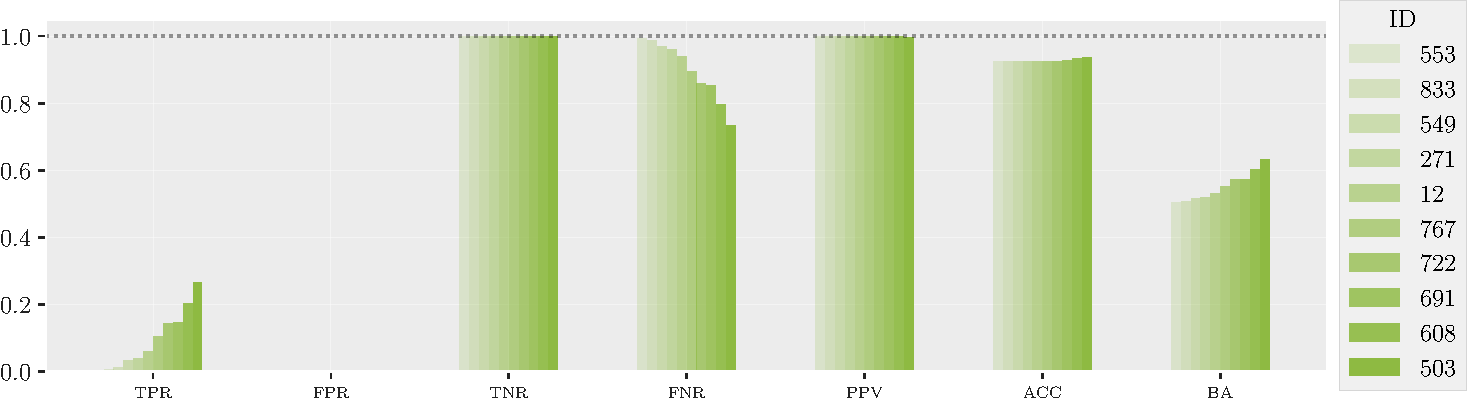
\includegraphics[width=\textwidth]{build/metrics_fact.pdf}
    \caption{Metrics for \fact{}. The cleaning setting with ID~947 performs
    best in terms of the number of true positives, accuracy and balanced accuracy, making it the best
    setting of the nine parameter combinations.}
    \label{fig:metrics_fact}
\end{figure}

\begin{table}
    \centering
    \caption{Results for the metrics of \tcc{}. The best results are obtained
    with the setting with ID~1954.}
    \label{tab:metrics_tcc}
    \rowcolors{0}{white!92!black}{}
    \begin{tabular}{r S[table-format=1.4] S[table-format=1.4] S[table-format=1.4] S[table-format=1.4] S[table-format=1.4] S[table-format=1.4] S[table-format=1.4] }
        \hiderowcolors
        ID & \acrshort{tpr} & \acrshort{tnr} & \acrshort{fnr} & \acrshort{acc} & \acrshort{ba} \\
        \addlinespace[0.5em]
        \showrowcolors
        % \input{build/metrics_tcc.txt}
          11 & 0.0452 & 1.0000 & 0.9548 & 0.9256 & 0.5226 \\
         367 & 0.0717 & 1.0000 & 0.9283 & 0.9256 & 0.5359 \\
         399 & 0.1071 & 1.0000 & 0.8929 & 0.9256 & 0.5535 \\
         582 & 0.1403 & 1.0000 & 0.8597 & 0.9267 & 0.5701 \\
         171 & 0.1653 & 1.0000 & 0.8347 & 0.9278 & 0.5827 \\
        1495 & 0.2088 & 1.0000 & 0.7912 & 0.9321 & 0.6044 \\
         807 & 0.2314 & 1.0000 & 0.7686 & 0.9364 & 0.6157 \\
        1954 & 0.3065 & 0.9998 & 0.6935 & 0.9418 & 0.6531 \\
    \end{tabular}
\end{table}

\begin{figure}
    \centering
    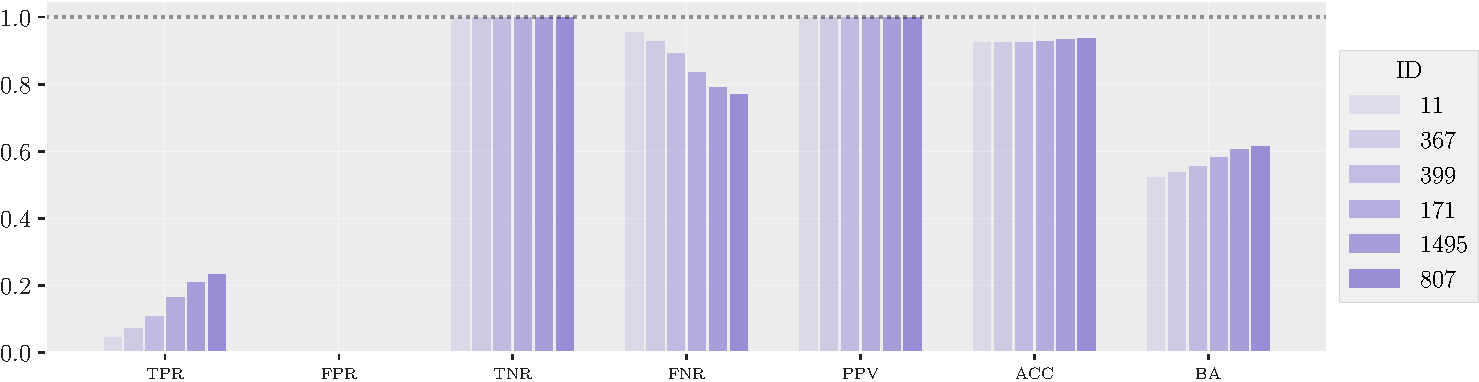
\includegraphics[width=\textwidth]{build/metrics_tcc.pdf}
    \caption{Metrics for the \tcc{}. The cleaning setting with ID~1954 performs
    best in terms of the number of true positives, accuracy and balanced accuracy, making it the best
    setting of the eight parameter combinations.}
    \label{fig:metrics_tcc}
\end{figure}

\begin{table}
    \centering
    \caption{Best-performing IDs \wrt the metrics and the corresponding hyperparameters for each respective cleaner.
    Listed are the core threshold \(Q_c\), the boundary threshold \(Q_b\),
    the minimum number of neighbors and, where applicable, the time limit \(t\) as well as the core and boundary time limits
    \(t_c\) and \(t_b\).}
    \label{tab:best_parameters}
    \rowcolors{0}{white!92!black}{}
    \begin{tabular}{c S[table-format=2.0] S[table-format=1.3]
        S[table-format=1.3] S[table-format=1.0] S[table-format=2.1] S[table-format=2.1] S[table-format=2.1]}
        \hiderowcolors
        {Cleaning Algorithm} & {ID} & {\(Q_c \;/\; \si{\pe}\)} & {\(Q_b \;/\; \si{\pe}\)} & {Min. Neigh.} &
        {\(t \;/\; \si{\nano\second}\)} & {\(t_c \;/\; \si{\nano\second}\)} & {\(t_b \;/\; \si{\nano\second}\)} \\
        \addlinespace[0.5em]
        \showrowcolors
        \tailcuts &  101 & 6.700 & 1.675 & 1 &      &      &      \\
        \mars     &   13 & 5.500 & 1.833 & 2 &      &      &      \\
        \fact     &  974 & 4.200 & 1.400 & 2 &  6.0 &      &      \\
        \tcc      & 1954 & 6.700 & 1.675 & 1 &      & 15.0 &  9.0 \\
    \end{tabular}
\end{table}

\section{Performance Compared to the Default Settings}
\label{sec:performance}

Now, with a setting selected for each cleaner, it is reasonable to compare
the performance to the default settings, that are implemented in the \ctapipe{} source code
(see \autoref{tab:hyperparameters}). First, the relative angular resolution
\begin{equation}
    \theta_{\SI{68}{\percent},\,\text{rel}} = \frac{\theta_{\SI{68}{\percent}}}{\theta_{\SI{68}{\percent},\,\text{base}}}
\end{equation}
is computed for the default (base) settings and the selected settings for each cleaner.
The results are shown in \autoref{fig:rel_angres} for the same efficiency intervals
as in \autoref{fig:efficiency_angres}. One can see, that especially for the interval
\([0.40, 0.45)\) and at medium to high energies, \tcc{} performs fairly well compared to the default settings.
The other algorithms perform only slightly better than the default settings at a performance gain
of up to \(\SI{50}{\percent}\) \eg for \mars{}. Notably for \mars{} is how it performs consistently
across the whole energy range.

Furthermore, the metrics of the hyperparameters determined in this work can be compared to the
metrics of the default settings. The results are shown in \autoref{fig:metrics_comparison} with the
values of the metrics being listed in \autoref{tab:metrics_default}. The values for the selected
settings in this work are listed in \autoref{tab:metrics_all}.
With the hyperparameters found in this work, all four algorithms perform better than with the default
settings. Especially \tcc{} and \tailcuts{} and \mars{} gain a significant improvement, most notably in the \gls{tpr} and
\gls{ba} scores. The improvement for \tcc{} is even more notable than for \mars{} and \tailcuts{}.\fact{}
also improved in terms of the \gls{tpr} and \gls{acc}, but not as much as the rest.

\begin{figure}
    \centering
    \includegraphics[width=\textwidth]{build/metrics_baseline.pdf}
    \caption{Metrics for the default (baseline) settings compared to the settings determined in this work.
    One can see that a significant improvement was reached for \tcc{} and \tailcuts{} and \mars{}, especially in terms of \gls{tpr} and \gls{ba}.
    \fact{} did only slightly improve, especially in terms of \gls{acc}.}
    \label{fig:metrics_comparison}
\end{figure}
\begin{figure}
    \centering
    \begin{subfigure}[t]{0.45\textwidth}
        \centering
        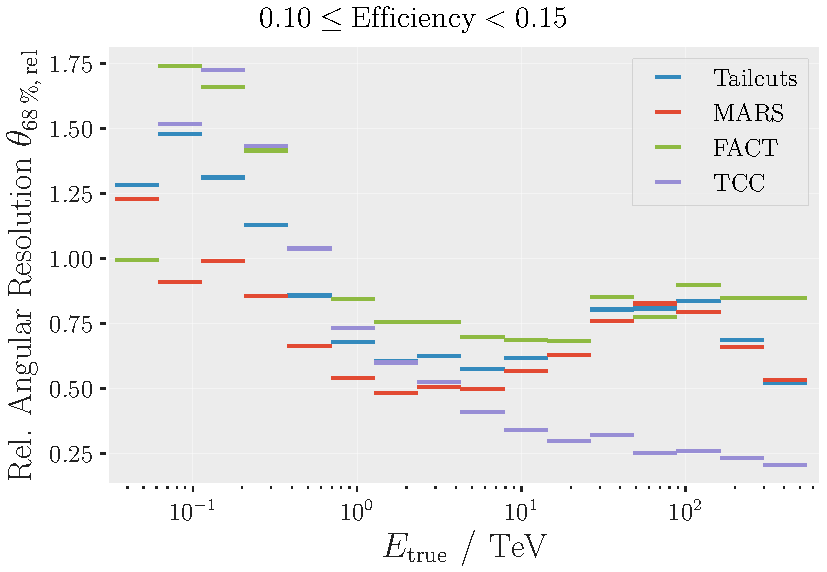
\includegraphics[width=\textwidth]{plots/ar_aeff/Rel_AR_0.10_0.15_base.pdf}
    \end{subfigure}
    \hfill
    \begin{subfigure}[t]{0.45\textwidth}
        \centering
        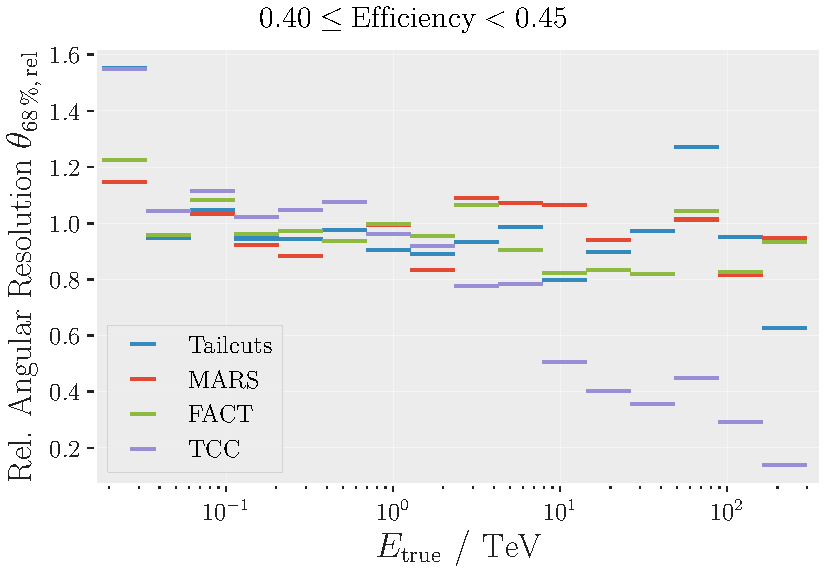
\includegraphics[width=\textwidth]{plots/ar_aeff/Rel_AR_0.40_0.45_base.pdf}
    \end{subfigure}
    \caption{Relative angular resolution for the default settings and the selected settings for each cleaner.
    \tcc{} outperforms the default values with the new settings, especially at higher energies. \mars{} seems
    to perform fairly consistently across the whole energy range, followed by \tailcuts{}. \fact{} performs
    consistently for higher energies.}
    \label{fig:rel_angres}
\end{figure}

\begin{table}
    \centering
    \caption{Metrics for the default (baseline) settings. The found hyperparameters listed in
    \autoref{tab:best_parameters} improve the performance of each cleaner over the default settings.
    Especially \tcc{} and \tailcuts{} gained better scores \wrt the metrics.}
    \label{tab:metrics_default}
    \rowcolors{0}{white!92!black}{}
    \begin{tabular}{c S[table-format=1.4] S[table-format=1.4] S[table-format=1.4]
        S[table-format=1.4] S[table-format=1.4] S[table-format=1.4] S[table-format=1.4]}
        \hiderowcolors
        {Cleaning Algorithm} & {\acrshort{tpr}} & {\acrshort{tnr}} &
        {\acrshort{fnr}} & {\acrshort{acc}} & {\acrshort{ba}} \\
        \addlinespace[0.5em]
        \showrowcolors
        \tailcuts & 0.2316 & 1.0000 & 0.7684 & 0.9358 & 0.6158 \\
        \mars     & 0.2346 & 1.0000 & 0.7654 & 0.9358 & 0.6173 \\
        \fact     & 0.3261 & 0.9998 & 0.6739 & 0.9429 & 0.6629 \\
        \tcc      & 0.1790 & 1.0000 & 0.8210 & 0.9299 & 0.5895 \\

    \end{tabular}
\end{table}

\section{Comparison of the Cleaning Algorithms}
\label{sec:comparison}

As of writing this thesis, the cleaning algorithms discussed in this thesis are the only ones implemented
in the \ctapipe{} source code. With the determined hyperparameters, I decided to compare the performance of all
four cleaners. I once again decided to use the settings selected in \autoref{sec:metrics} for each algorithm
and look at the metrics. The metrics of all four algorithms are shown in \autoref{fig:metrics_all}.
The corresponding values are listed in \autoref{tab:metrics_all}.

One can see, that \fact{} performs best out of all algorithms \wrt the metrics, closely followed by \mars{}.
Both algorithms perform well in terms of \gls{tpr} and \gls{ba}. \tailcuts{} and \tcc{}, although performing
slightly worse than \fact{} and \mars{}, still perform fairly well. Both have the same scores for the \gls{acc}
and a similar score for the \gls{ba}.
\begin{table}
    \centering
    \caption{Metrics for the selected settings of each cleaning algorithm. Out of these
    four algorithms, \fact{} performs best in terms of \gls{tpr} and \gls{ba} with \mars{}
    and following closely. \tailcuts{} and \tcc{}, although slightly worse than the other two,
    still perform fairly well. \mars{}, due to its consistency for the angular resolution, is
    a viable alternative to \fact{}.}
    \label{tab:metrics_all}
    \rowcolors{0}{white!92!black}{}
    \begin{tabular}{c S[table-format=1.4] S[table-format=1.4] S[table-format=1.4]
        S[table-format=1.4] S[table-format=1.4] S[table-format=1.4] S[table-format=1.4]}
        \hiderowcolors
        {Cleaning Algorithm} & {\acrshort{tpr}} & {\acrshort{tnr}} &
        {\acrshort{fnr}} & {\acrshort{acc}} & {\acrshort{ba}} \\
        \addlinespace[0.5em]
        \showrowcolors
        \tailcuts & 0.3169 & 0.9997 & 0.6831 & 0.9418 & 0.6583 \\
        \mars     & 0.3460 & 0.9995 & 0.6540 & 0.9684 & 0.6727 \\
        \fact     & 0.3493 & 0.9996 & 0.6507 & 0.9687 & 0.6745 \\
        \tcc      & 0.3065 & 0.9998 & 0.6935 & 0.9418 & 0.6531 \\
    \end{tabular}
\end{table}

\begin{figure}
    \centering
    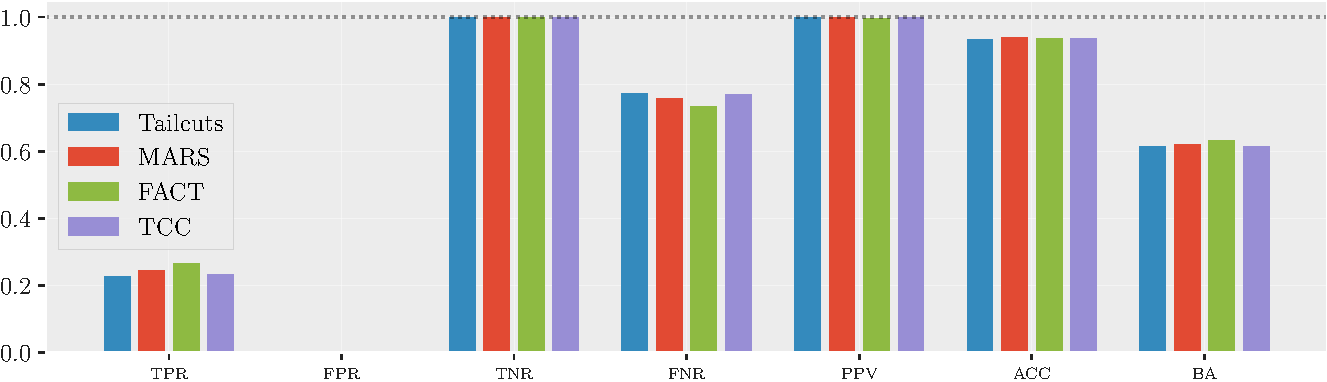
\includegraphics[width=\textwidth]{build/metrics_all.pdf}
    \caption{Bar plot visualizing the metrics for the selected settings of all four cleaning algorithms.
    \fact{} performs best out of all cleaning algorithms, followed by \mars{}. The latter, however
    performs consistently \wrt the angular resolution, as shown in \autoref{fig:rel_angres} and can therefore be considered
    a viable alternative to \fact{}. \tailcuts{} and \fact{} perform slightly worse than the other two, but still fairly well.}
    \label{fig:metrics_all}
\end{figure}